\documentclass[UTF8]{article}
\usepackage{ctex}
\usepackage[margin=1in]{geometry}
\usepackage[colorlinks,linkcolor=blue]{hyperref} 
\usepackage{graphicx}
\usepackage{amsmath}

\begin{document}
\title{Automated Essay Scoring Report}
\author{MF1933059 刘冀 MF1933061 刘猛 MG1933088 袁佳莉}
\date{January 2020}
\maketitle

本篇报告是对文章自动评分课程作业三次实验的的总结报告。本小组一共有三名同学:刘冀,刘猛,袁佳莉。
在这三次实验中,我们分别设计和实现了多个模型,实现了每个成员的结果提交,并采用最优结果作为小组
提交结果。本篇报告整体分为三个部分,分别对应三次实验。

\section{第一次实验}

第一次实验是在 Prompt-dependent 的条件下,基于统计方法去分别预测八个类别文章的分数,需要手动设计特征。

\subsection{特征设置}

本次实验中我们一共尝试构建了两组特征用于实现文档向量化,分别由两位组员独立设计与实现,
下面我们分别介绍两组特征。

\subsubsection{第一组特征}

第一组特征一共包含 16 个文档特征:
\begin{itemize}
    \item 文章中单词、句子的平均长度(2个)
    \item 文章中单词长度、句子长度的方差(2个)
    \item 文章的字符、单词、句子的频数(3个)
    \item 文章中副词、介词、逗号的频数(3个)
    \item 文章中拼写错误单词的个数(1个)
    \item 文章中句子的平均子句个数、平均子句长度、最大子句个数、最长子句长度(4个)
    \item 文章中只出现过一次的单词的个数(1个)
\end{itemize}

以上 16 个特征是通过调用 NLTK 和 StanfordNLP 以及 pyenchant 第三方语言处理库
来构建的,具体实现过程可以参考\href{https://github.com/Mandule/EssayAE/tree/master/HW1}{代码}。

\subsubsection{第二组特征}
第二组特征一共包含 15 个文档特征:

\begin{itemize}
    \item 文章中单词、句子的平均长度(2个)
    \item 文章中单词长度、句子长度的方差(2个)
    \item 文章的字符、单词、句子的频数(3个)
    \item 文章中介词、逗号的频数(3个)
    \item 文章中拼写错误单词的个数(1个)
    \item 文章中句子的平均子句个数、平均子句长度(2个)
    \item 文章中只出现过一次的单词的个数(1个)
    \item 文章中句子语法树平均深度(1个)
    \item 文章中句子语法树平均叶节点深度(1个)
\end{itemize}

以上 16 个特征是通过调用 NLTK 和 StanfordNLP 以及 pyspellchecker 第三方语言处理库
来构建的。

\subsection{实验设置}

\begin{figure}[h]
    \centering
    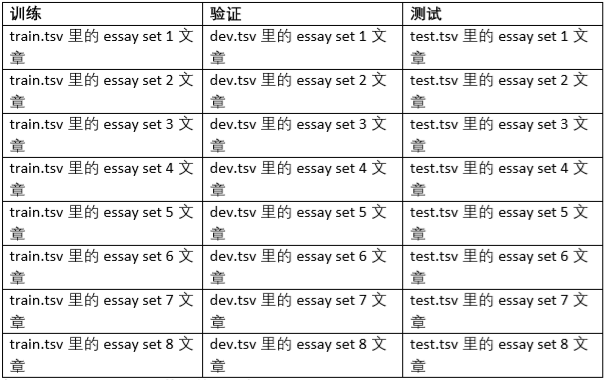
\includegraphics[width=0.7\textwidth]{fig/11.png}
    \caption{数据集划分}
    \label{fig:HW1}
\end{figure}

数据集划分如图\ref{fig:HW1}所示。

本小节将会介绍本次实验流程的设置,主要分为一下五个步骤:
\begin{enumerate}
    \item 文章数据预处理

    分词、分句,去除停用词,去除非英文单词标识符。
    \item 文章向量化
    
    分别使用上一小节构建的两组特征进行向量化,通过实验分析两组特征对性能的影响。
    \item 训练 SVC,SVR
    
    按照图\ref{fig:HW1}中的数据集划分,训练8个SVC和8个SVR。
    \item 性能评估
    
    利用验证集上的Kappa值评估两组特征的性能。

    利用验证集上的Kappa值评估SVC,SVR的性能。
    \item 结果提交
    
    根据性能评估的结果,选择最优的一组特征用于文章向量化,并选用最优的学习算法产生测试集结果。
\end{enumerate}

实验环境:python-3.7.5,nltk-3.4.5,pandas-0.25.3,numpy-1.17.3,pyenchant-2.0.0 pyspellchecker-0.5.3

\subsection{实验结果与分析}

本次实验中,我们组将重心放在了构建特征上,最终在每个类别的文章数据集
中选用最优学习算法(SVC或SVR)产生测试结果。

\begin{itemize}
    \item 特征组一:0.69
    \item 特征组二:0.71
\end{itemize}

通过两组特征的对比分析,可以发现语法树中的统计信息对文章自动评分任务的性能有显著提高。可以想象这是符合
老师判卷的标准,如果一个学生使用的语句语法更加复杂,修辞和转折更多的话,那么该学生的分数可能也会更高。

最终我们选择使用第二组特征并结合使用SVC和SVR学习器产生测试集结果。

\textbf{提交结果为0.7114333565031952,最终排名在10-20内。}

\subsection{总结}

在利用统计学习方法解决文章自动评分的实验中,我们将重心放在了特征的构建和抽取上,并使用简单的分类或回归算法
进行测试。我们意识到如果使用更复杂的学习算法(XGBoosting,LightGBM等)可能会取得更优的结果,但是我们经过
讨论决定不使用此类学习器进行实验,因为不想将整个实验过程变为疯狂调参的过程。实验结果证明,我们构建的特征即使
在简单的学习器上也能取得较好的效果。

通过对实验中构建的两组特征的对比,我们可以得出这样一个结论:句子级别的语法特征和文章的分数相关性较高。
通过回归任务和分类任务的对比,我们可以得出这样一个结论:文章自动评分任务更适合作为回归任务来处理。

\section{第二次实验}
第二次实验的任务和第一次实验的任务相同,但是本次实验将使用深度神经网络来进行建模,利用端到端
的训练方法来完成文章自动评分任务。本章将主要报告我们组在模型构建方面的构思与实践,简化模型训练
过程中的调参技巧。

\subsection{模型设置}
在本次实验中我们一共设计和实现了两个深度模型,分别由两位组员独立设计和实现,
下面我们将分别介绍这两个模型的结构。

\subsubsection{Transformer}
鉴于Transformer强有力的特征抽取能力,我们设计了一个简单的基于TransformerEncoder的网络来完成文章自动评分任务。

\begin{figure}[h]
    \centering
    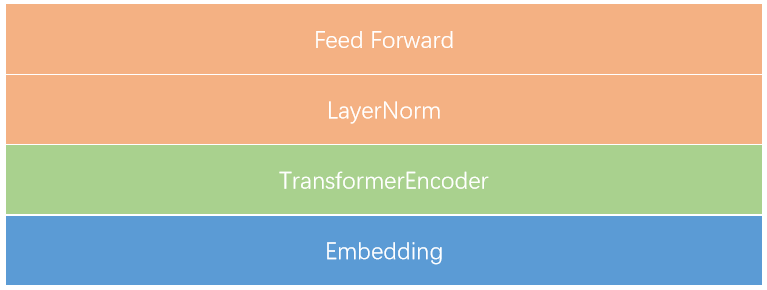
\includegraphics[width=0.7\textwidth]{fig/5.png}
    \caption{Transformer}
    \label{fig:Transformer}
\end{figure}

如图\ref{fig:Transformer}所示,Embedding层使用的是维度为50的Glove预训练词向量。Transformer利用多头注意力机制
对输入的文章进行特征提取,并送入前馈神经网络输入文章的预测分数。

\subsubsection{CNN-LSTM}

在设计CNN-LSTM 模型之前,我们尝试使用 Bi-LSTM 模型,但是提交的结果并不理想,所以我们决定在
Bi-LSTM 的基础之上进行改进。基于第一次实验的经验,我们可以得出结论:句子级别的信息对文章的分数
有很大的影响,Bi-LSTM 并不能很好的对句子级别的信息进行建模,所以我们打算使用分层的信息抽取结构。

CNN-LSTM 是一种分层的深度神经网络,其基本思想是先使用 CNN 对文章中每个句子进行处理,得到一个定长的句子向量,
再将文章中的所有句子向量作为 Bi-LSTM 的输入最后得到定长的文章向量。模型的设计思想虽然简单,但是实现过程
比单纯使用 Bi-LSTM 复杂了很多,性能也得到了显著地提升。

下面将主要介绍模型的结构,主要分为两个部分:Inception,Bi-LSTM。

\begin{figure}[h]
    \centering
    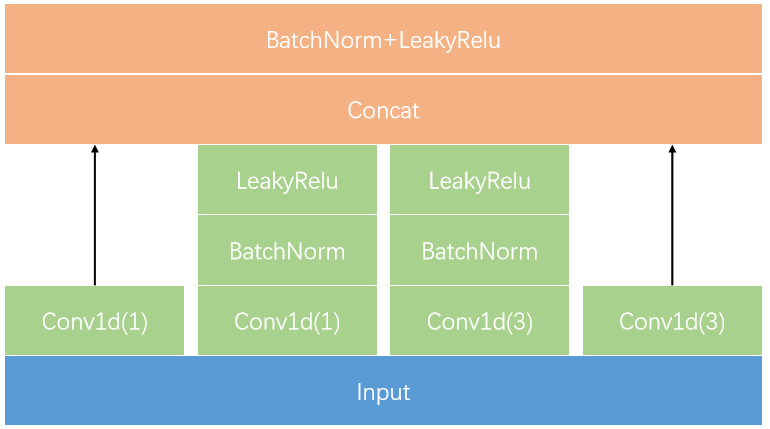
\includegraphics[width=0.7\textwidth]{fig/1.png}
    \caption{Inception}
    \label{fig:Inception}
\end{figure}

图\ref{fig:Inception}展示了句子级 Inception 的结构,该结构借鉴了经典网络
\href{https://arxiv.org/pdf/1512.00567.pdf}{Google Inception Net}的思想,
使用了四个一维卷积核进行特征提取,本质上是提取了句子中的N-gram信息,
本次实验中使用了2个Inception块的叠加作为句子级别的 CNN 网络结构。Embedding层使用
的是维度为300的Glove预训练词向量,并且在训练过程中锁定不更新。

\begin{figure}[h]
    \centering
    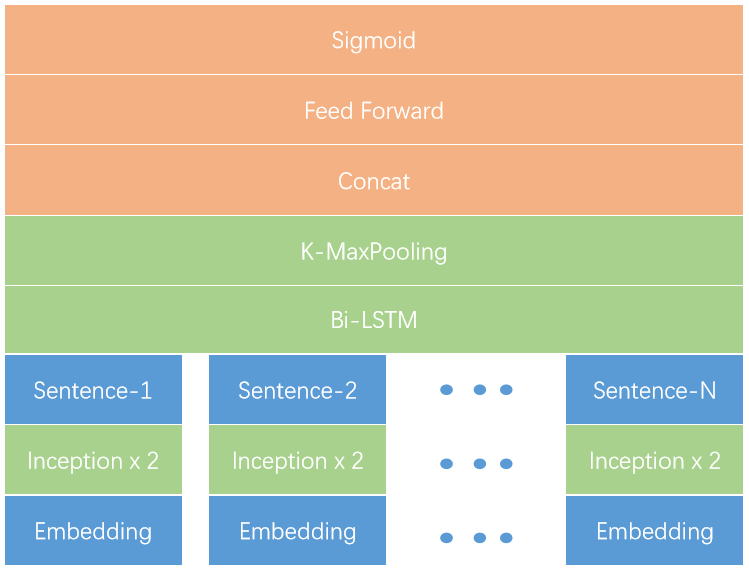
\includegraphics[width=0.65\textwidth]{fig/2.png}
    \caption{CNN-LSTM}
    \label{fig:CNN-LSTM}
\end{figure}

图\ref{fig:CNN-LSTM}展示了 CNN-LSTM 模型的结构。
该网络由两层 Inception 结构和 Bi-LSTM组成,使用 KMaxPooling 取 k 个状态输出
的拼接作为前馈神经网络的输入,最后输出的是一个(0,1)区间内的值,该值作为文章的预测得分。
具体的实现可以参考\href{https://github.com/Mandule/EssayAE/tree/master/HW2}{代码}。

\subsection{实验设置}

\begin{figure}[h]
    \centering
    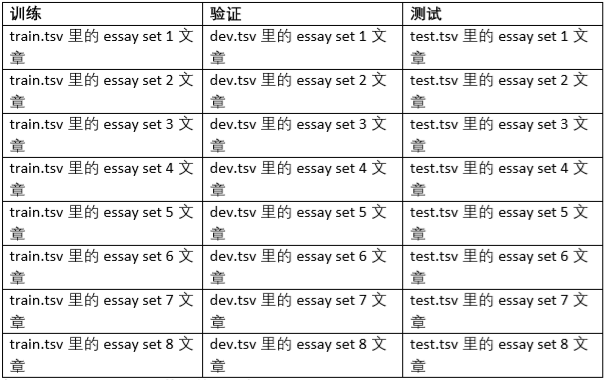
\includegraphics[width=0.7\textwidth]{fig/11.png}
    \caption{数据集划分}
    \label{fig:HW2}
\end{figure}

数据集划分如图\ref{fig:HW2}所示。

前小节已经介绍了Transformer 模型和CNN-LSTM的模型结构,本小节将会介绍本次实验的过程,
主要分为一下五个步骤:
\begin{enumerate}
    \item 文章数据预处理

    分词、分句,去除停用词,去除非英文单词标识符。还有注意的一点就是要将文章的评分归一化到(0,1)区间。
    \item 加载数据
    
    由于深度模型的训练每次需要使用一批数据,所以我们需要自定义DataSet来实现模型对输入数据的格式需求。
    Transformer和CNN-LSTM由两位不同的组员设计并实现,所以各自定义了各自的DataSet和DataLoader,具体可以参考代码。
    \item 训练模型
    
    两位组员分别训练八个Transformer模型和八个CNN-LSTM模型并保存在本地,对应于八个文章类别,
    目的是比较模型的性能。
    \item 性能评估
    
    利用验证集上的Kappa值评估两个模型在八个文章类别上的性能。需要注意的是,在性能评估时需要将(0,1)的
    文章分数通过运算转化为该类别对应的分数范围。
    \item 结果提交
    
    根据性能评估的结果,加载性能最优的模型用于预测测试集的结果。
\end{enumerate}

实验环境:python-3.7.5,nltk-3.4.5,pandas-0.25.3,numpy-1.17.3,pytorch-1.3.1

\subsection{实验结果与分析}

本次实验中,我们组将重心放在了深度模型的设计和实现上,最终在每个类别的文章数据集
中选用最优模型产生测试集预测结果。

\begin{itemize}
    \item Transformer:0.73
    \item CNN-LSTM:0.76
\end{itemize}

通过两个模型的对比我们可以分析出,CNN-LSTM虽然使用的是循环神经网络,但是分层的网络结构使得模型可以捕捉到
更好的句子级别的语义信息,对于文章的评分起了关键作用。如果将循环神经网络替换为TransformerBlock的结构,
可能性能会有进一步的提升。

最终我们选择使用CNN-LSTM作为预测最终结果的模型。

\textbf{提交结果为0.7628964065829837,最终排名在10-20内。}

\subsection{总结}

在基于深度神经网络的文章自动评分实验中,我们将重心放在了深度模型的构建上,尝试了Transformer结构和
简单的 Bi—LSTM 和CNN-LSTM 的复杂结构,模型的实现是很简单的,我们相对花了更多的时间在数据的处理上。

我们意识到直接使用大型预训练模型(BERT等)可能会取得更优的结果,同第一次实验一样我们并未使用
最暴力的调参解决方案,而是从零开始尝试构建一个深度模型用于解决文章自动评分任务。
实验证明,每次模型的改进都带了准确率的提升,并且最终取得了较为不错的性能,基于时间因素,模型还有很多
需要改进的地方。

本次实验中,CNN-LSTM 取得了最优结果,在未进行大量调参尝试的情况下,使用0.001的初始学习率和Adam优化器
进行了epoch=50轮的训练,最终提交结果为 0.7628964065829837,最终排名在10-20名。

通过本次实验我们总结出了几点经验:
\begin{itemize}
    \item 模型的设计需要结合特定的任务。
    \item 文本分析任务中数据的处理是非常重要的。
    \item 循环神经网络使用orthogonal初始化效果会更好。
    \item 过拟合非常普遍,要在模型中添加合适的Drop层。
\end{itemize}

CNN-LSTM 模型的实现和训练过程具体参考\href{https://github.com/Mandule/EssayAE/tree/master/HW2}{代码}。

\section{第三次实验}

第三次实验室跟前两次的实验不同,需要在 promp-independent 条件下对未在训练集中的文章进行评分。
实验要求使用除目标文章类别以外的七个文章类别作为训练集,以目标文章类别作为测试集。
本章将主要报告我们组在模型构建方面的构思与实践,简化模型训练过程中的调参技巧。

\subsection{模型设置}

本次实验中我们一共设计了两个模型,分别由两个组员独立设计与实现,下面我们将分别介绍两个模型的结构。

\subsubsection{1D-CNN}
1D-CNN尝试用简单的一维卷积神经网络来完成文章自动评分任务。图\ref{fig:1DCNN}是1D-CNN的模型结构
示意图,该模型使用多层的一维卷积操作进行特征提取。

\begin{figure}[h]
    \centering
    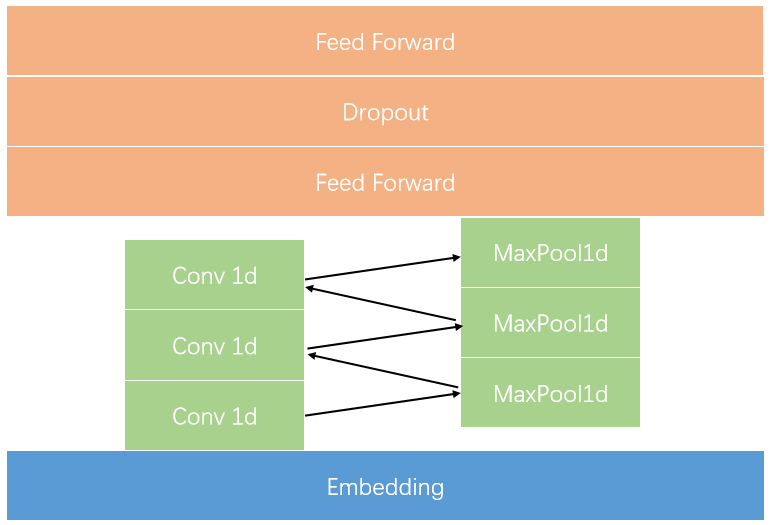
\includegraphics[width=0.7\textwidth]{fig/3.png}
    \caption{1D-CNN}
    \label{fig:1DCNN}
\end{figure}

\subsubsection{Prompt-CNN-LSTM}

Prompt-CNN-LSTM 模型是基于第二次实验中提出的 CNN-LSTM 模型,我们又单独增加了个一个主题模块,输入
是每一类文章的 Prompt,输出为一个定长向量,用于提取 Prompt 的信息。Prompt 的定长向量将会同 CNN-LSTM 
输出的文章向量拼接后输入到前馈神经网络中。

该模型设计的主要思想是,文章的得分一共基于两个方面:学生的文笔,文章的扣题程度。一篇文章只有文笔好,并且准确
扣题才可能获得高分,所以我们认为有必要将 Prompt 的信息利用起来。实验证明,加入了 Prompt 信息后,模型的准确
率有了大幅提升。

\begin{figure}[h]
    \centering
    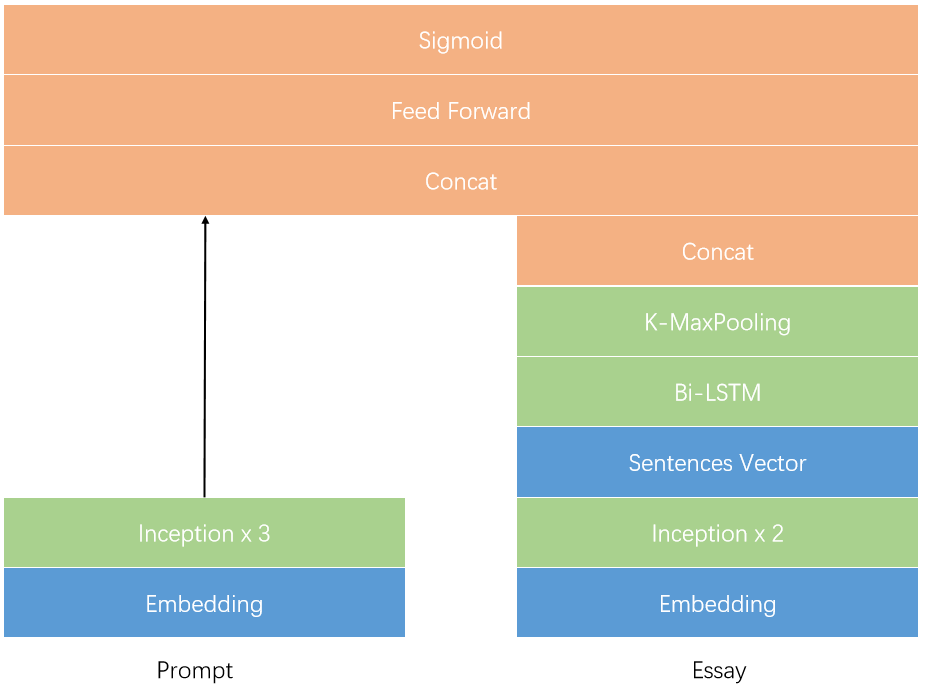
\includegraphics[width=0.7\textwidth]{fig/4.png}
    \caption{Prompt-CNN-LSTM}
    \label{fig:Prompt}
\end{figure}

如图\ref{fig:Prompt}所示,左侧模块的输入为 Prompt,右侧模块的输入是第二次实验中的CNN-LSTM 模型,最后将
两个模块的输出进行拼接后输入到前馈网络中,得到文章在其特定主题下的得分(0,1)。
Inception的结构如图\ref{fig:Inception}所示,Prompt 模块仅使用了三层 Inception 模块的叠加,
较为简单,这是考虑到每个 prompt 的长度并不长,所以没有
使用更复杂的网络结构。模型的具体实现可以参考\href{https://github.com/Mandule/EssayAE/tree/master/HW3}{代码}。

\subsection{实验设置}

\begin{figure}[h]
    \centering
    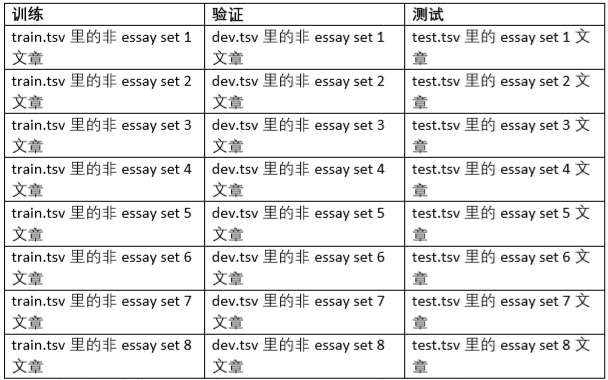
\includegraphics[width=0.7\textwidth]{fig/22.png}
    \caption{数据集划分}
    \label{fig:HW3}
\end{figure}

数据集划分如图\ref{fig:HW3}所示。需要注意的是,本次实验预测的文章是不存在于训练集中的。

前小节已经介绍了1D-CNN模型和Prompt-CNN-LSTM模型,本小节将会介绍本次实验的过程,主要分为一下五个步骤:
\begin{enumerate}
    \item 文章数据预处理

    分词、分句,去除停用词,去除非英文单词标识符。还有注意的一点就是要将文章的评分归一化到(0,1)区间。
    \item 加载数据
    
    由于深度模型的训练每次需要使用一批数据,所以我们需要自定义DataSet来实现模型对输入数据的格式需求。
    1D-CNN和prompt-CNN-LSTM由两位不同的组员设计并实现,所以各自定义了各自的DataSet和DataLoader,具体可以参考代码。
    需要注意的是,prompt-CNN-LSTM由于用到了八个类别 prompt 信息,所以会多加载一部分数据,具体实现可以参考
    \href{https://github.com/Mandule/EssayAE/tree/master/HW3}{代码}。
    \item 训练模型
    
    两位组员分别训练八个1D-CNN模型和八个CNN-LSTM模型并保存在本地,对应于八个文章类别,
    目的是比较模型的性能。
    \item 性能评估
    
    利用验证集上的Kappa值评估两个模型在八个文章类别上的性能。需要注意的是,在性能评估时需要将(0,1)的
    文章分数通过运算转化为该类别对应的分数范围。
    \item 结果提交
    
    根据性能评估的结果,加载性能最优的模型用于预测测试集的结果。
\end{enumerate}

实验环境:python-3.7.5,nltk-3.4.5,pandas-0.25.3,numpy-1.17.3,pytorch-1.3.1

\subsection{实验结果与分析}

本次实验中,我们组将重心放在了深度模型的设计和实现上,最终在每个类别的文章数据集
中选用最优模型产生测试集预测结果。

\begin{itemize}
    \item 1D-CNN:0.46
    \item prompt-CNN-LSTM:0.64
\end{itemize}

通过对比两个模型的性能,我们可以分析出,单纯使用CNN对文章进行建模是远远不够的,CNN和LSTM的结合会带来
性能的显著提升。引入 prompt 信息是可以显著增加性能的,这很符合老师判卷时的标准,如果一个学生写的文章
不扣题,那么很可能会被判零分。prompt-CNN-LSTM 考虑了主题和文章的关系,虽然设计的结构很简单但是一定程度上
捕捉了两者的联系,所以性能得到了提升。

最终我们选择使用prompt-CNN-LSTM作为预测最终结果的模型。

\textbf{提交结果为0.6476745212774347,最终排名在10-20内。}

\subsection{总结}

本次实验中,我们将重心放在了对第二次实验的模型的改进上,引入了 Prompt 信息,这对于性能的提升至关重要。
第三次实验时间仓促,没有做更多的改进和优化,其实模型本身还存在很多缺陷,例如没有使用attention机制,prompt
信息的建模过于简单等等。

本次实验中,prompt-CNN-LSTM 取得了最优结果,在未进行大量调参尝试的情况下,使用0.001的初始学习率和Adam优化器
进行了epoch=50轮的训练,最终提交结果为 0.6476745212774347,最终排名在10-20名。

prompt-CNN-LSTM 模型的实现和训练过程具体参考\href{https://github.com/Mandule/EssayAE/tree/master/HW3}{代码}。

\section{报告总结}

本次报告分三个部分,总结了三次实验的设计思路、模型结构、实验流程、实验结果、实验分析等内容,较为全面的介绍了我们组
在本次课程中的学习成果。

三次实验的最优结果和排名:
\begin{itemize}
    \item 第一次实验:0.7114333565031952    10-20名
    \item 第二次实验:0.7628964065829837    10-20名
    \item 第三次实验:0.6476745212774347    10-20名
\end{itemize}

可以看到我们的排名并不是非常靠前,这是由于我们的每次实验都是从零开始自己探索和学习,并未使用任何高性能的
预训练模型,这是为了避免三次实验陷入疯狂调参的局面,这样就失去了学习自然语言课程的乐趣。通过三次实验的实践,
我们对自然语言处理有了进一步理解。

\section{组员信息与分工}

\begin{itemize}
    \item 刘冀  MF1933059
    \item 刘猛  MF1933061
    \item 袁佳莉    MG1933088
\end{itemize}

三个组员在三次实验中的工作如图\ref{fig:分工}所示,红色代表最优结果。

\begin{figure}[h]
    \centering
    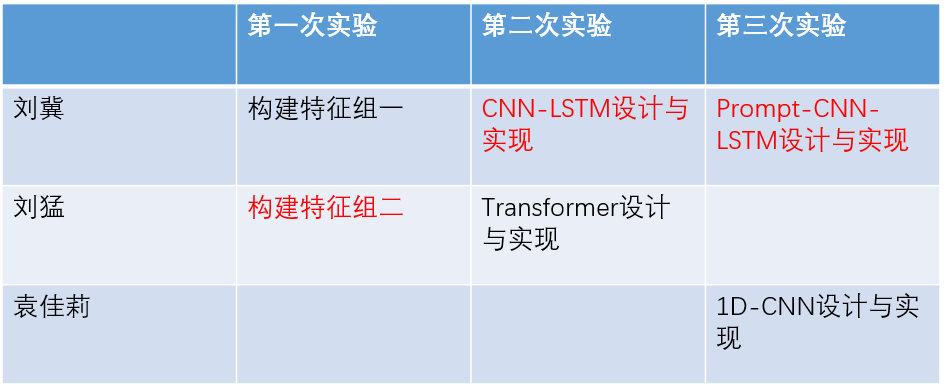
\includegraphics[width=0.7\textwidth]{fig/6.png}
    \caption{组员分工}
    \label{fig:分工}
\end{figure}



\end{document}